\documentclass[aspectratio=169]{beamer}
\usetheme{Madrid}
\usecolortheme{default}

% Packages
\usepackage[utf8]{inputenc}
\usepackage{graphicx}
\usepackage{amsmath}
\usepackage{amsfonts}
\usepackage{amssymb}
\usepackage{hyperref}
\usepackage{tikz}
\usepackage{pgfplots}
\usepackage{listings}
\usepackage{xcolor}
\usepackage{booktabs}
\usepackage{multirow}
\usepackage{subcaption}

% Custom colors
\definecolor{teslaBlue}{RGB}{33, 150, 243}
\definecolor{aiGreen}{RGB}{76, 175, 80}
\definecolor{warningOrange}{RGB}{255, 152, 0}
\definecolor{errorRed}{RGB}{244, 67, 54}

% Title information
\title[Physical AI \& LLMs in Autonomous Driving]{Physical AI and Large Language Models in Autonomous Driving}
\subtitle{A Comprehensive Technical Overview}
\author{Technical Presentation}
\institute{Based on comprehensive research document}
\date{\today}

% Custom commands
\newcommand{\highlight}[1]{\textcolor{teslaBlue}{\textbf{#1}}}
\newcommand{\advantage}[1]{\textcolor{aiGreen}{\checkmark\ #1}}
\newcommand{\limitation}[1]{\textcolor{errorRed}{\times\ #1}}

\begin{document}

% Title slide
\begin{frame}
    \titlepage
\end{frame}

% Table of Contents
\begin{frame}{Agenda}
    \tableofcontents
\end{frame}

% Section 1: Introduction
\section{Introduction: The Convergence}

\begin{frame}{The Convergence of Physical AI and LLMs}
    \begin{block}{Revolutionary Transformation}
        The autonomous driving landscape is undergoing a \highlight{revolutionary transformation} through the integration of:
    \end{block}
    
    \begin{columns}
        \begin{column}{0.5\textwidth}
            \begin{itemize}
                \item \textbf{Physical AI}: AI systems that perceive and interact with the physical world
                \item \textbf{Large Language Models}: Advanced reasoning and natural language capabilities
            \end{itemize}
        \end{column}
        \begin{column}{0.5\textwidth}
            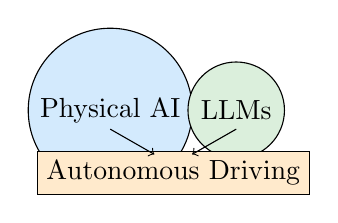
\begin{tikzpicture}[scale=0.8]
                \node[draw, circle, fill=teslaBlue!20] at (0,1) {Physical AI};
                \node[draw, circle, fill=aiGreen!20] at (2,1) {LLMs};
                \node[draw, rectangle, fill=warningOrange!20] at (1,0) {Autonomous Driving};
                \draw[->] (0,0.7) -- (0.7,0.3);
                \draw[->] (2,0.7) -- (1.3,0.3);
            \end{tikzpicture}
        \end{column}
    \end{columns}
    
    \vspace{0.5cm}
    This convergence creates intelligent, adaptive frameworks that can understand, reason, and interact with the physical world.
\end{frame}

\begin{frame}{From Rule-Based to Intelligent Systems}
    \begin{columns}
        \begin{column}{0.5\textwidth}
            \begin{block}{Traditional Systems}
                \begin{itemize}
                    \item Pre-programmed rules
                    \item Pattern recognition
                    \item Limited adaptability
                    \item Rigid responses
                \end{itemize}
            \end{block}
        \end{column}
        \begin{column}{0.5\textwidth}
            \begin{block}{Physical AI + LLMs}
                \begin{itemize}
                    \item Contextual understanding
                    \item Natural language interaction
                    \item Adaptive learning
                    \item Nuanced decision making
                \end{itemize}
            \end{block}
        \end{column}
    \end{columns}
\end{frame}

% Section 2: Why Physical AI & LLMs Matter
\section{Why Physical AI \& LLMs are Crucial}

\begin{frame}{5 Key Advantages}
    \begin{enumerate}
        \item \highlight{Contextual Understanding \& Reasoning}
        \item \highlight{Multimodal Perception \& Integration}
        \item \highlight{Adaptive Learning \& Generalization}
        \item \highlight{Safety \& Explainability}
        \item \highlight{Human-Centric Design}
    \end{enumerate}
\end{frame}

\begin{frame}{1. Contextual Understanding \& Reasoning}
    \begin{itemize}
        \item \textbf{Natural Language Instructions}
            \begin{itemize}
                \item \textit{"Take me to the hospital, it's an emergency"}
            \end{itemize}
        \item \textbf{Complex Scenarios}
            \begin{itemize}
                \item Construction zones, emergency vehicles, unusual patterns
            \end{itemize}
        \item \textbf{Human-AI Interaction}
            \begin{itemize}
                \item Natural communication about preferences and concerns
            \end{itemize}
    \end{itemize}
\end{frame}

\begin{frame}{2. Multimodal Perception \& Integration}
    \begin{columns}
        \begin{column}{0.5\textwidth}
            \textbf{Sensor Modalities:}
            \begin{itemize}
                \item Visual Cameras (RGB, IR, depth)
                \item LiDAR (3D point clouds)
                \item Radar (weather-resistant)
                \item Audio (environmental + passenger)
                \item GPS \& IMU (location + motion)
            \end{itemize}
        \end{column}
        \begin{column}{0.5\textwidth}
            \textbf{Integration Benefits:}
            \begin{itemize}
                \item Unified environment understanding
                \item Contextual interpretation
                \item Robust perception
                \item Enhanced decision making
            \end{itemize}
        \end{column}
    \end{columns}
\end{frame}

\begin{frame}{3. Adaptive Learning \& Generalization}
    \begin{itemize}
        \item \textbf{Few-shot Learning}: Adapt to new conditions with minimal examples
        \item \textbf{Transfer Learning}: Apply knowledge across domains
        \item \textbf{Continuous Improvement}: Learn from real-world experiences
    \end{itemize}
\end{frame}

\begin{frame}{4. Safety \& Explainability}
    \begin{itemize}
        \item \textbf{Explain Decisions}
            \begin{itemize}
                \item \textit{"I'm slowing down because I detected a child's ball rolling into the street"}
            \end{itemize}
        \item \textbf{Predict Intentions}: Understanding behavior patterns
        \item \textbf{Handle Edge Cases}: Reasoning through unprecedented scenarios
    \end{itemize}
\end{frame}

\begin{frame}{5. Human-Centric Design}
    \begin{itemize}
        \item \textbf{Natural Communication}: Voice-based passenger interaction
        \item \textbf{Personalization}: Learning individual preferences
        \item \textbf{Accessibility}: Supporting diverse user needs
    \end{itemize}
\end{frame}

% Section 3: Current Solutions
\section{Current Solutions in Autonomous Driving}

\begin{frame}{Current Solutions Overview}
    Evolution through several technological approaches, each building upon previous innovations.
    
    \vspace{0.5cm}
    \begin{center}
        \textbf{References:} arXiv:2003.06404, IEEE 9304823
    \end{center}
\end{frame}

\begin{frame}{The "4 Pillars" Architecture}
    Traditional modular, linear system with sequential processing:
    
    \vspace{0.5cm}
    \begin{center}
        \texttt{Sensors → Perception → Localization → Planning → Control → Actuation}
    \end{center}
    
    \vspace{0.5cm}
    \begin{figure}
        \centering
        \includegraphics[width=0.8\textwidth]{docs/figures/autonomous4pillars.png}
        \caption{4 Pillars Architecture}
    \end{figure}
\end{frame}

\begin{frame}{The Four Pillars Explained (1/2)}
    \begin{columns}
        \begin{column}{0.5\textwidth}
            \textbf{1. Perception Pillar}
            \begin{itemize}
                \item Object detection \& classification
                \item Lane detection \& road segmentation
                \item Traffic sign recognition
                \item Depth estimation \& 3D reconstruction
            \end{itemize}
        \end{column}
        \begin{column}{0.5\textwidth}
            \textbf{2. Localization Pillar}
            \begin{itemize}
                \item GPS + IMU integration
                \item SLAM (Simultaneous Localization and Mapping)
                \item HD map matching
                \item Sensor fusion for positioning
            \end{itemize}
        \end{column}
    \end{columns}
\end{frame}

\begin{frame}{The Four Pillars Explained (2/2)}
    \begin{columns}
        \begin{column}{0.5\textwidth}
            \textbf{3. Planning Pillar}
            \begin{itemize}
                \item Route planning (global)
                \item Behavior planning (tactical)
                \item Motion planning (local)
                \item Trajectory optimization
            \end{itemize}
        \end{column}
        \begin{column}{0.5\textwidth}
            \textbf{4. Control Pillar}
            \begin{itemize}
                \item Longitudinal control (speed)
                \item Lateral control (steering)
                \item PID controllers
                \item Model Predictive Control (MPC)
            \end{itemize}
        \end{column}
    \end{columns}
\end{frame}

\begin{frame}{Industry Variations}
    \begin{columns}
        \begin{column}{0.5\textwidth}
            \textbf{Waymo Approach}
            \begin{itemize}
                \item Heavy reliance on LiDAR
                \item Detailed HD maps
                \item Geofenced operations
                \item Rule-based decision making
            \end{itemize}
        \end{column}
        \begin{column}{0.5\textwidth}
            \textbf{Baidu Apollo}
            \begin{itemize}
                \item Open-source platform
                \item Modular architecture
                \item Cloud-based HD mapping
                \item Simulation-first development
            \end{itemize}
        \end{column}
    \end{columns}
\end{frame}

\begin{frame}{Advantages \& Limitations}
    \begin{columns}
        \begin{column}{0.5\textwidth}
            \textbf{Advantages}
            \begin{itemize}
                \item[\textcolor{aiGreen}{✓}] Interpretable and debuggable
                \item[\textcolor{aiGreen}{✓}] Modular development
                \item[\textcolor{aiGreen}{✓}] Proven in controlled environments
                \item[\textcolor{aiGreen}{✓}] Safety through redundancy
            \end{itemize}
        \end{column}
        \begin{column}{0.5\textwidth}
            \textbf{Limitations}
            \begin{itemize}
                \item[\textcolor{errorRed}{✗}] Error propagation through pipeline
                \item[\textcolor{errorRed}{✗}] Limited adaptability
                \item[\textcolor{errorRed}{✗}] High computational overhead
                \item[\textcolor{errorRed}{✗}] Difficulty handling edge cases
            \end{itemize}
        \end{column}
    \end{columns}
\end{frame}

\begin{frame}{Open Source Implementations}
    \begin{itemize}
        \item \textbf{Apollo by Baidu}: Complete autonomous driving platform
        \item \textbf{Autoware}: Open-source software for autonomous driving
        \item \textbf{OpenPilot by Comma.ai}: Open source driver assistance system
        \item \textbf{CARLA Simulator}: Open-source simulator for autonomous driving research
        \item \textbf{AirSim}: Simulator for drones, cars and more
    \end{itemize}
\end{frame}

% Section 4: Tesla Case Study
\section{Tesla's Latest Model: A Case Study}

\begin{frame}{Tesla's Full Self-Driving System}
    Tesla's Full Self-Driving (FSD) system represents one of the most advanced implementations of neural network-based autonomous driving.
    
    \vspace{0.5cm}
    \begin{center}
        \textbf{Reference:} thinkautonomous.ai/blog/tesla-end-to-end-deep-learning
    \end{center}
\end{frame}

\begin{frame}{Evolution from Modular to End-to-End}
    Tesla's system has undergone significant architectural transformation:
    
    \begin{itemize}
        \item \textbf{2019-2020}: HydraNet (Multi-task learning)
        \item \textbf{2021}: Combined Perception + Planning
        \item \textbf{2022}: Addition of Occupancy Networks
        \item \textbf{2023+}: Full End-to-End Learning (FSD v12)
    \end{itemize}
\end{frame}

\begin{frame}{Key Architectural Differences}
    \begin{table}[h]
        \centering
        \small
        \begin{tabular}{@{}lll@{}}
            \toprule
            \textbf{Aspect} & \textbf{Modular Architecture} & \textbf{End-to-End Architecture} \\
            \midrule
            Data Flow & Sequential pipeline & Direct sensor-to-action \\
            Optimization & Component-wise & Joint optimization \\
            Error Handling & Error propagation & Global error correction \\
            Adaptability & Limited & High adaptability \\
            \bottomrule
        \end{tabular}
    \end{table}
\end{frame}

\begin{frame}{Vision Transformer (ViT) Architecture}
    Tesla's perception system leverages Vision Transformers for:
    
    \begin{itemize}
        \item \textbf{Global Context}: Processes entire image patches simultaneously
        \item \textbf{Multi-Camera Fusion}: Attention mechanisms handle relationships between camera views
        \item \textbf{Temporal Understanding}: Self-attention across time enables motion prediction
    \end{itemize}
\end{frame}

\begin{frame}{Occupancy Networks}
    Enhanced perception with 3D occupancy prediction:
    
    \begin{itemize}
        \item Converts image space into voxels with free/occupied classification
        \item Provides dense spatial understanding for static and dynamic objects
        \item Enhances context understanding in 3D space
    \end{itemize}
\end{frame}

% Section 5: Future Directions
\section{Future Research Directions}

\begin{frame}{Future Research Directions}
    The convergence of Physical AI and LLMs opens exciting possibilities for autonomous driving.
\end{frame}

\begin{frame}{Emerging Trends}
    \begin{itemize}
        \item \textbf{Multimodal Foundation Models}: Unified models handling vision, language, and action
        \item \textbf{Embodied AI}: AI systems that understand physical world interactions
        \item \textbf{Causal Reasoning}: Understanding cause-and-effect relationships in driving scenarios
        \item \textbf{Few-Shot Adaptation}: Rapid adaptation to new environments and conditions
    \end{itemize}
\end{frame}

\begin{frame}{Technical Challenges}
    \begin{itemize}
        \item \textbf{Real-time Processing}: Balancing model complexity with latency requirements
        \item \textbf{Safety Guarantees}: Ensuring reliable performance in safety-critical scenarios
        \item \textbf{Data Efficiency}: Learning from limited labeled data
        \item \textbf{Interpretability}: Understanding model decisions for regulatory compliance
    \end{itemize}
\end{frame}

\begin{frame}{Research Opportunities}
    \begin{itemize}
        \item \textbf{Sim-to-Real Transfer}: Bridging the gap between simulation and real-world performance
        \item \textbf{Human-AI Collaboration}: Seamless handover between human and AI control
        \item \textbf{Ethical AI}: Addressing bias and fairness in autonomous decision making
        \item \textbf{Federated Learning}: Privacy-preserving learning across vehicle fleets
    \end{itemize}
\end{frame}

% Section 6: Conclusion
\section{Conclusion}

\begin{frame}{Conclusion}
    The integration of \highlight{Physical AI} and \highlight{Large Language Models} represents a transformative approach to autonomous driving.
    
    \vspace{0.5cm}
    \textbf{Key takeaways:}
    \begin{itemize}
        \item Evolution from rule-based to intelligent, adaptive systems
        \item Multimodal perception enables richer understanding
        \item End-to-end learning shows promising results
        \item Human-centric design improves accessibility and usability
        \item Significant research opportunities remain
    \end{itemize}
\end{frame}

\begin{frame}
    \begin{center}
        \Huge Thank You
        
        \vspace{1cm}
        \Large Questions \& Discussion
    \end{center}
\end{frame}

\end{document}